\section{Grundlagen}
\label{sec:grundlagen}
In diesem Versuch werden verschiedene Schaltungen mit Hilfe des
Operationsverstärkers realisiert.
Zunächst wird auf die physikalischen Eigenschaften eingegangen,
woraufhin verschiedene Schaltungen skizziert und schließlich
realisiert werden.

\subsection{Eigenschaften des Operationsverstärkers}
\label{subsec:eigenschaften}
Die wichtigste elektrische Eigenschaft des Operationsverstärkers
ist die Proportionalität der Ausgangsspannung $U_\text{A}$ zur
Differenz der Eingangsspannungen $U_\text{p}$ und $U_\text{N}$:
\begin{equation}
\label{eq:proportionalität}
    U_\text{A} = V(U_\text{p} - U_\text{N})\,,
\end{equation}
wobei $V$ die Leerlaufverstärkung bezeichnet.
Diese Beziehung gilt in einem Spannungsbereich
$-U_\text{B} < U_\text{A} < U_\text{B}$, der durch die Betriebsspannung
$U_\text{B}$ bestimmt ist. Ausserhalb dieses Bereichs läuft die
Ausgangsspannung in eine Sättigung.
Die Eingangsspannung $U_\text{p}$ wird nicht invertiert, während die Spannung
$U_\text{N}$ invertiert wird -- der Verstärker besitzt also einen
nicht-invertierenden und einen invertierenden Eingang.

Aus technischer Sicht entspricht der Operationsverstärker einem
gleichstromgekoppeltem Differenzverstärker. Er ist in Abbildung
\ref{fig:op} dargestellt.
\begin{figure}
    \centering
    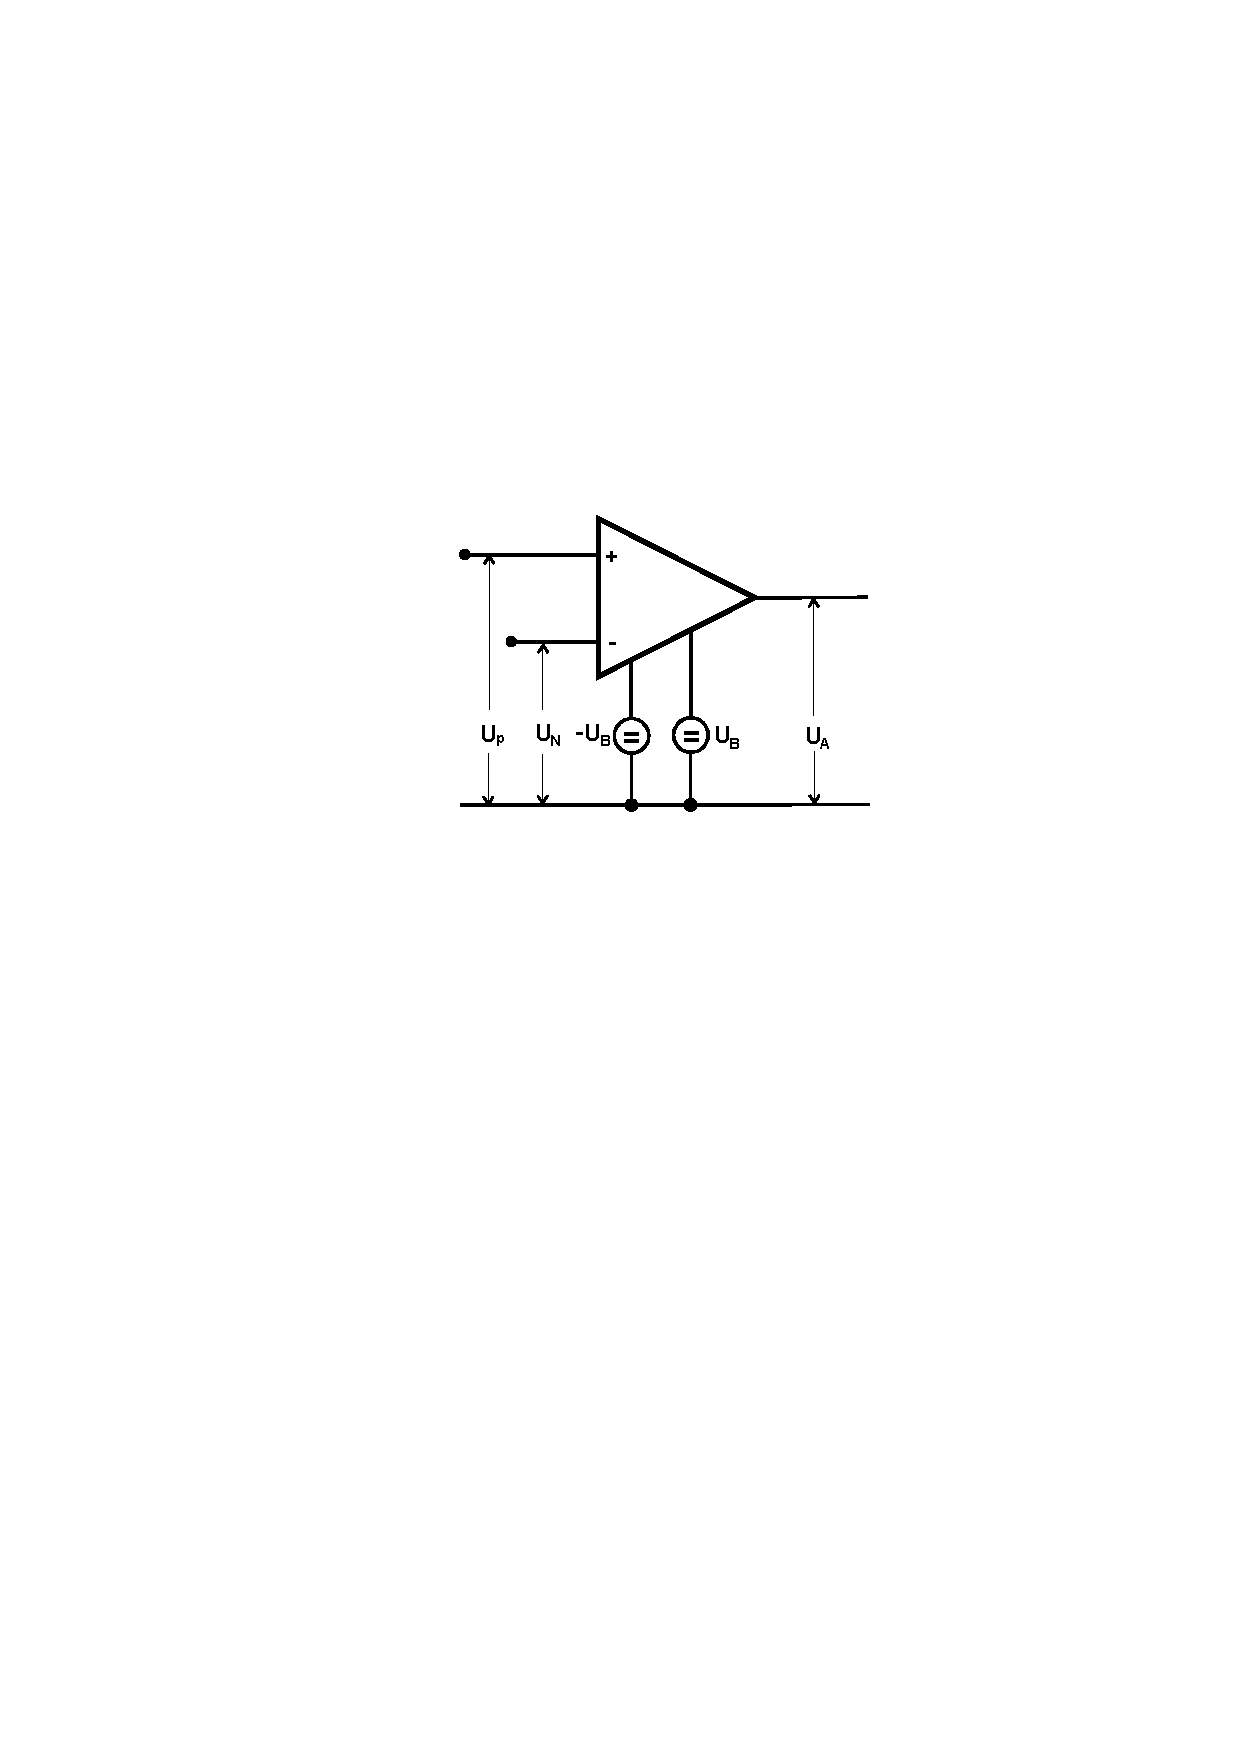
\includegraphics[width=0.7\linewidth]{img/op.pdf}
    \caption{
        Schaltbild eines Operationsverstärkers mit Ausgangsspannung
        $U_\text{A}$ und Eingangsspannungen $U_\text{p}$ und
        $U_\text{N}$ \cite{V51}.
    }
    \label{fig:op}
\end{figure}
Neben der meist frequenzabhängigen Leerlaufverstärkung $V$ besitzt der
Operationsverstärker weitere Kenngrößen, wie die Eingangswiderstände,
$r_\text{e,p}$ und $r_\text{e,N}$, sowie 
einen Ausgangswiderstand $r_\text{a}$.
Um Rechnungen zu Vereinfachen gilt für einen idealen Operationsverstärker
\begin{equation}
\label{eq:id-verstärker}
    V = \infty\,,\qquad r_\text{e} = \infty\,,\qquad r_\text{a} = 0\,.
\end{equation}

Im Gegensatz dazu müssen zur theoretischen Beschreibung eines realen
Operationsverstärkers zusätzliche Kenngrößen in Betracht gezogen werden.

Die Gleichtaktverstärkung
\begin{equation}
\label{eq:gleichtaktverstärkung}
    V_\text{Gl} = \frac{\Delta U_\text{A}}{\Delta U_\text{Gl}}
\end{equation}
berücksichtigt geringe Asymmetrien der beiden Vertärkungskanäle.
Dabei bezeichnen $\Delta U_\text{A}$ die Differenz der Ausgangsspannung zu
\num{0} und $\Delta U_\text{Gl}$ den Unterschied der -- eigentlich gleichen --
Eingangsspannungen.

Die auf Grund endlicher Eingangswiderstände $r_\text{e}$ auftretenden
Eingangsströme werden mit $I_\text{p}$ und $I_\text{N}$, deren
Mittelwert,
\begin{equation}
\label{eq:eingangsruhestrom}
    I_\text{B} = \frac{1}{2}\left(I_\text{p} + I_\text{N}\right)\,,
\end{equation}
als Eingangsruhestrom und die Differenz
\begin{equation}
\label{eq:offsetstrom}
    I_\text{B} = \frac{1}{2}\left(I_\text{p} + I_\text{N}\right)\,,
\end{equation}
als Offsetstrom bezeichnet.
Ähnlich zum Offsetstrom, verschwindet auch die Spannung häufig nicht.
Für die Offsetspannung $U_0$ gilt daher bei $U_\text{A} = 0$
\begin{equation}
\label{eq:offsetspannung}
    U_0 = U_\text{t} - U_\text{N}\,.
\end{equation}
Sie ist abhängig von Temperatur, Zeit und Betriebsspannungen. Die totale
Ableitung wird mit Offsetspannungsdrift bezeichnet.


\section{Schaltungsbeispiele}
\label{sec:schaltungsbeispiele}
Im Folgenden werden einige Schaltbeispiele für Operationsverstärker
dargestellt. Das Verhalten des Verstärkers hängt dabei meist nur von der
äußeren Schaltung ab und kann damit als annähernd ideal angenommen werden.

\subsection{Rückgekoppelter Linearverstärker}
\label{subsec:rück-linearverstärker}
Der relativ kleine Arbeitsbereich des Operationsverstärkers ist in der
Anwendung oft nicht praktikabel. Um diesen Bereich zu verbreitern, wird die
Verstärkung reduziert, indem ein Teil der Ausgangsspannung auf den
invertierenden Eingang gegeben wird.
Der Anteil der zurückgeführten Spannung kann dabei mit Hilfe der Widerstände
$R_1$ und $R_\text{N}$ bestimmt werden, die in Abbildung \ref{fig:linear}
dargestellt sind.
\begin{figure}
    \centering
    \includegraphics[width=0.7\linewidth]{img/linearverstärker.pdf}
    \caption{Rückgekoppelter Linearverstärker \cite{V51}.}
    \label{fig:linear}
\end{figure}
Für den Fall $R_\text{N}/R_1 \ll V$
lässt sich zeigen, dass die Verstärkung $V^\prime$ nur noch vom Verhältnis
dieser beiden Widerstände abhängt.
Der Geringe Eingangswiderstand $r_\text{e} \approx R_1$ wirkt sich bei
hochohmigen Spannungsquellen möglicherweise nachteilig aus. Im nächsten
Abschnitt wird daher ein Linearverstärker vorgestellt, der diesen Nachteil
umgeht.

\subsection{Elektrometerverstärker}
\label{subsec:elektrometerverstärker}
Wie in Abbildung \ref{fig:elektrometer} deutlich wird, wird auch bei diesem
Verstärker ein Teil der Ausgangsspannung $U_\text{A}$ zum gegengekoppelten
Eingang zurückgeführt. Dabei sind die Widerstände $R_1$ und $R_\text{N}$ auf
eine andere Art und Weise verschaltet, dass der Eingangswiderstand in der
Größenordnung des Gleichtakteingangwiderstandes
($r_\text{Gl} \approx \SI{10}{\giga\ohm}$) liegt.
\begin{figure}
    \centering
    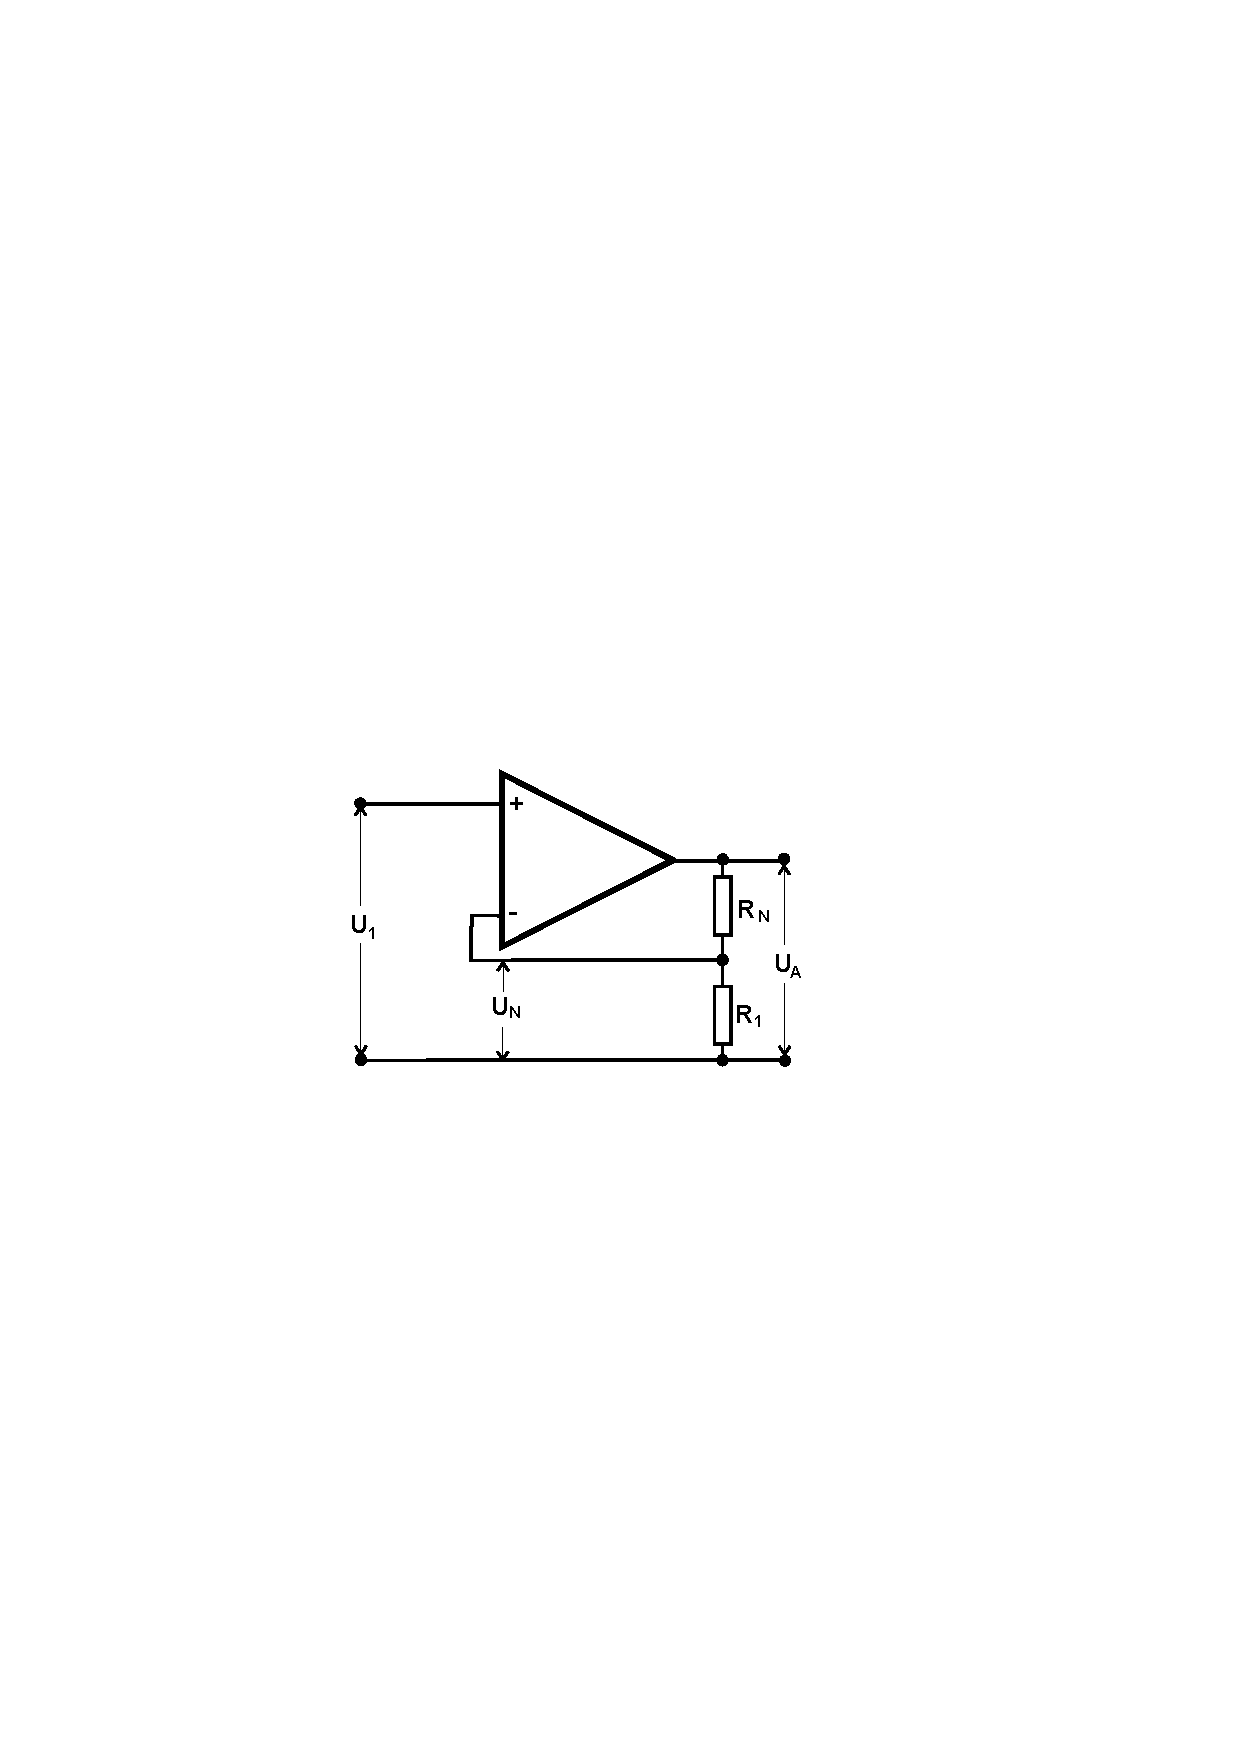
\includegraphics[width=0.7\linewidth]{img/elektrometer.pdf}
    \caption{Schaltbild eines Elektrometerverstärkers \cite{V51}.}
    \label{fig:elektrometer}
\end{figure}
